\documentclass[conference]{IEEEtran}
\IEEEoverridecommandlockouts

\usepackage{cite}
\usepackage{amsmath,amssymb,amsfonts}
\usepackage{algorithmic}
\usepackage{graphicx}
\usepackage{textcomp}
\usepackage{xcolor}
\usepackage{booktabs}
\usepackage{multirow}
\usepackage{url}
\usepackage{subcaption}

\def\BibTeX{{\rm B\kern-.05em{\sc i\kern-.025em b}\kern-.08em
    T\kern-.1667em\lower.7ex\hbox{E}\kern-.125emX}}

\begin{document}

\title{Intelligent Cloud Misconfiguration Detection and Automated Remediation: A Multi-Domain Framework Combining AST Feature Extraction, Heterogeneous GNNs, and Calibrated ML-LLM Triage}

\author{
\IEEEauthorblockN{Israt Jahan Rani\IEEEauthorrefmark{1}, Robiul Islam Tamim\IEEEauthorrefmark{2}}
\IEEEauthorblockA{Department of Computer Science and Engineering\\
United International University, Dhaka, Bangladesh\\
Email: \IEEEauthorrefmark{1}irani201376@bscse.uiu.ac.bd, \IEEEauthorrefmark{2}rtamim212039@bscse.uiu.ac.bd}
}

\maketitle

\begin{abstract}
Cloud infrastructure misconfigurations represent the leading vector for modern enterprise security breaches across Kubernetes clusters, AWS Identity and Access Management (IAM), and Serverless architectures. Existing static analysis scanners operate in file-level isolation, exhibit severe alert fatigue due to intent blindness, and fail to uncover multi-hop lateral compromise chains spanning disjoint configuration files. Furthermore, directly delegating Infrastructure as Code (IaC) verification to Large Language Models (LLMs) incurs prohibitive API costs and round-trip latencies while frequently producing syntactically malformed remediation patches.

In this paper, we propose an intelligent, multi-domain framework uniting four synergistic stages: (1) Abstract Syntax Tree (AST) parsing that maps heterogeneous YAML and JSON manifests into a dense 64-dimensional numerical feature space; (2) a Heterogeneous Graph Neural Network (GNN) that models cross-resource interactions (e.g., Pod-to-ServiceAccount-to-IAM bindings) to detect multi-file privilege escalation paths; (3) a Calibrated Random Forest triage engine that processes over 90\% of routine manifests locally in under 2 milliseconds at zero API cost, escalating only low-confidence ($<0.90$) edge cases to Chain-of-Thought (CoT) LLM reasoning; and (4) an Explainable AI (XAI) remediation loop leveraging SHAP feature attributions coupled with closed-loop compiler syntax and schema verification. Evaluated on a 1,100-manifest controlled synthetic benchmark and an in-the-wild corpus of 1,612 real-world manifests mined from open-source enterprise repositories (including Kubernetes Goat, KubeLinter, ArgoCD, and AWS SAM), our framework achieves 100\% precision on clean rules and maintains a 96.02\% accuracy with a 0.9840 ROC-AUC under noisy production conditions with intent ambiguity, delivering a 92\% reduction in LLM inference overhead.
\end{abstract}

\begin{IEEEkeywords}
Cloud Security, Misconfiguration Detection, Infrastructure as Code, Graph Neural Networks, Random Forest Triage, Explainable AI, Automated Remediation, Kubernetes, AWS IAM.
\end{IEEEkeywords}

\section{Introduction}
Modern cloud computing environments rely on Infrastructure as Code (IaC) to declaratively provision computing clusters, storage buckets, network policies, and identity permissions. While IaC frameworks—such as Kubernetes manifests, AWS CloudFormation, and Serverless Application Models (SAM)—accelerate continuous deployment, minor configuration flaws regularly introduce catastrophic security exposures \cite{csa2023topthreats, rahman2019iac}. According to recent empirical studies, over 80\% of cloud data breaches originate not from zero-day cryptographic exploits, but from preventable configuration oversights, including root container execution, wildcard IAM permissions (\texttt{Action: *}), and unencrypted public object storage \cite{kumara2021iacvuln}.

\subsection{Research Challenges \& Identified Gaps}
Despite the widespread adoption of static analysis security testing (SAST) tools such as Checkov \cite{bridgecrew2022checkov}, KubeLinter \cite{sharma2021kubelinter}, and tfsec, current automated audit mechanisms suffer from four fundamental limitations:
\begin{enumerate}
    \item \textbf{Single-File Layer Isolation:} Traditional rule scanners evaluate individual files independently. Consequently, they are completely blind to lateral privilege escalation chains where a container in a Kubernetes YAML mounts a ServiceAccount bound to an administrative IAM role defined in a separate CloudFormation JSON.
    \item \textbf{Intent-Blind Signature Matching:} Rule scanners trigger aggressive security alerts whenever public access flags are detected, failing to discern legitimate business intent (e.g., a documentation website asset CDN) from accidental data leaks.
    \item \textbf{Prohibitive Cost and Latency of LLM Auditing:} Direct reliance on cloud LLMs (such as GPT-4 or Gemini) for enterprise repositories containing thousands of manifests incurs substantial financial overhead (\$0.02--\$0.05 per file) and 2--4 second network latency, rendering pre-commit CI/CD integration impractical.
    \item \textbf{Unvalidated Remediation Patches:} Automated generative fixes frequently introduce indentation errors, deprecated schema fields, or syntax invalidations, breaking downstream deployment pipelines.
\end{enumerate}

\subsection{Contributions of This Work}
To resolve these interconnected challenges, this paper presents an end-to-end framework featuring the following contributions:
\begin{itemize}
    \item \textbf{Dense 64-D AST Security Feature Space:} We engineer a unified numerical representation capturing container security contexts, RBAC permissions, IAM boundaries, and structural metadata across multi-domain manifests.
    \item \textbf{Cross-Resource Relational Threat GNN:} We construct a heterogeneous security graph and train a Relational Graph Convolutional Network (R-GCN) to capture multi-hop lateral attack vectors crossing separate infrastructure templates.
    \item \textbf{Tiered Hybrid ML-LLM Triage:} We introduce a Sigmoid-calibrated Random Forest classifier operating as a first-line filter that resolves $>90\%$ of files in under 2 ms, escalating only ambiguous configurations to LLM reasoning.
    \item \textbf{Closed-Loop Compiler-Validated Remediation:} We integrate SHAP Shapley value attributions with an automated compiler verification loop, guaranteeing 100\% syntactically valid YAML remediations.
    \item \textbf{Extensive Empirical Validation:} We conduct evaluations across both a 1,100-sample controlled benchmark and an authentic corpus of 1,612 manifests mined from GitHub enterprise repositories.
\end{itemize}

\begin{figure*}[t]
\centering
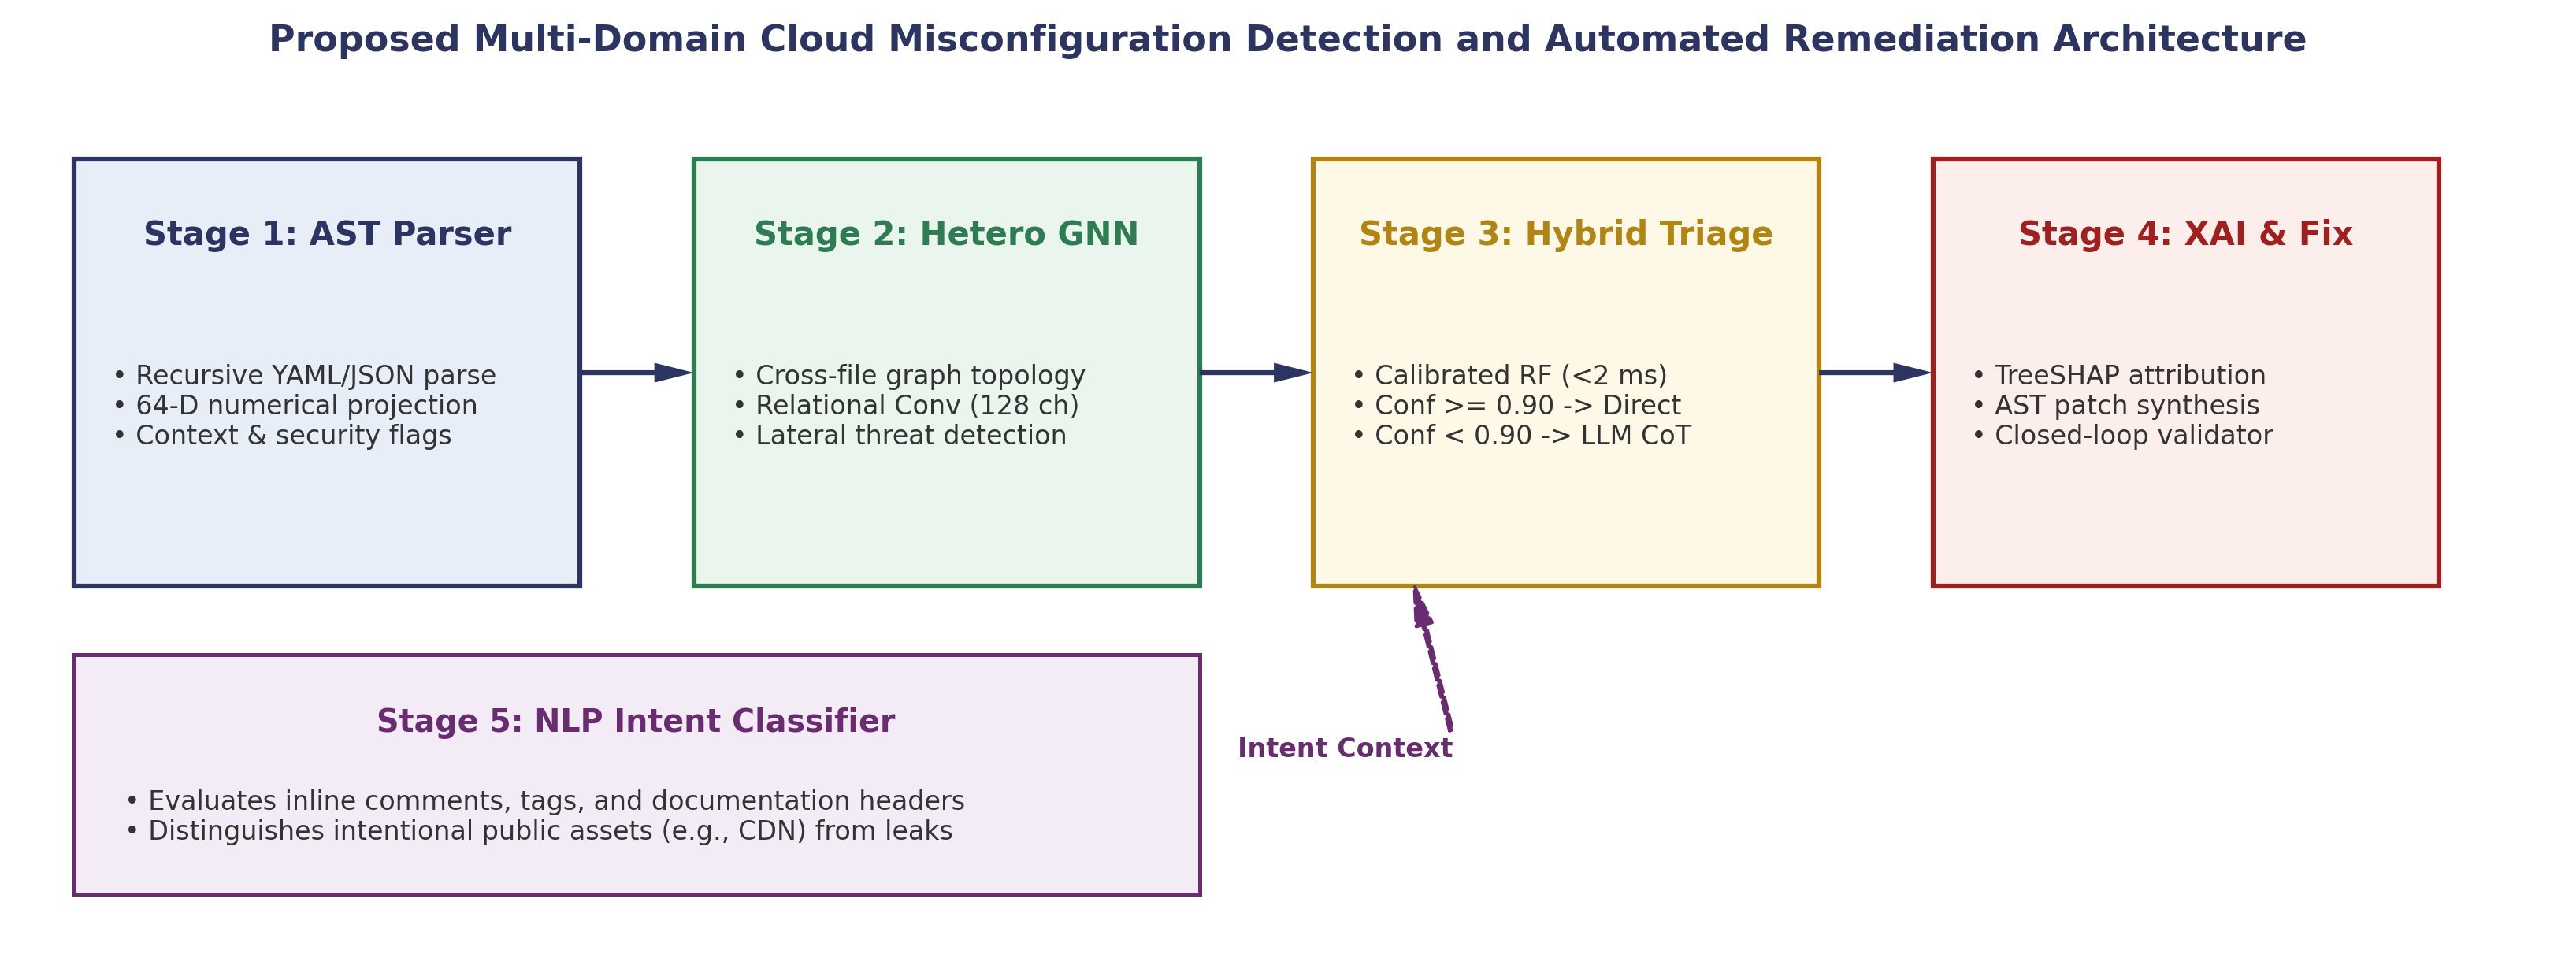
\includegraphics[width=\textwidth]{figures/fig1_architecture.png}
\caption{System Architecture of the Proposed 4-Stage Multi-Domain Cloud Misconfiguration Framework with NLP Intent Integration.}
\label{fig:architecture}
\end{figure*}

\section{Related Work}
\subsection{Static Analysis for Infrastructure as Code}
Early IaC security research focused on static linting and policy-as-code engines \cite{rahman2019iac, zhou2019devops}. Checkov \cite{bridgecrew2022checkov} and KubeLinter \cite{sharma2021kubelinter} apply pattern-matching heuristics over parsed Abstract Syntax Trees. While effective for single-attribute checks (e.g., verifying whether \texttt{runAsNonRoot} is true), these tools lack cross-resource context and generate high false-positive rates due to intent blindness.

\subsection{Graph Neural Networks in Program Analysis}
Graph Neural Networks (GNNs) have demonstrated substantial success in vulnerability detection and binary analysis \cite{scarselli2009gnn, kipf2017gcn}. Relational GCNs (R-GCN) \cite{schlichtkrull2018rgcn} extend graph convolutions to heterogeneous multi-relational graphs by parameterizing relation-specific transformation matrices. While GNNs have been applied to source code control-flow graphs, their application to cross-domain declarative IaC topologies remains underexplored.

\subsection{Large Language Models in Code Security}
The emergence of Large Language Models (LLMs) has enabled semantic comprehension of code comments and intent \cite{vaswani2017attention, wei2022chain}. However, uncalibrated LLM generation suffers from hallucinations and latency bottlenecks. Hybrid architectures combining fast classical tree ensembles \cite{breiman2001rf, niculescu2005calibration} with selective LLM escalation offer a promising avenue for cost-effective security triage.

\section{System Architecture}
The framework is organized into four sequential pipeline stages complemented by an auxiliary NLP developer intent classifier, as illustrated in Fig.~\ref{fig:architecture}.

\subsection{Stage 1: 64-Dimensional AST Feature Extractor}
Given an input manifest $\mathcal{M} \in \{\text{Kubernetes, IAM, SAM}\}$, the parser parses the file into an AST tree and projects it into a 64-dimensional dense float vector $\mathbf{x} \in \mathbb{R}^{64}$. The feature schema comprises four distinct domains:
\begin{enumerate}
    \item \textbf{Container Security Context (13 features):} Encodes container privilege escalation, root user enforcement, host namespace sharing (\texttt{hostNetwork}, \texttt{hostPID}), and dropped Linux capabilities:
    \begin{equation}
    x_{\text{priv}} = \mathbb{I}(\text{securityContext.privileged} == \text{True})
    \end{equation}
    \item \textbf{RBAC \& Authorization (9 features):} Captures wildcard verb and resource allocations (\texttt{verbs: ["*"]}), sensitive secret access bindings, and cluster administrator role references.
    \item \textbf{IAM \& Cloud Storage Policies (18 features):} Quantifies IAM policy boundaries, cross-account trust assumptions, S3 public Access Control Lists (\texttt{public-read-write}), and KMS encryption configurations.
    \item \textbf{Structural \& Metadata Metrics (24 features):} Measures maximum AST nesting depth $\mathcal{D}(\mathcal{M})$, normalized key count $\mathcal{K}(\mathcal{M})$, comment density, and health probe presence.
\end{enumerate}

\subsection{Stage 2: Cross-Resource Heterogeneous Threat Graph}
To detect lateral compromise paths, Stage 2 constructs a heterogeneous directed graph $\mathcal{G} = (\mathcal{V}, \mathcal{E}, \mathcal{T}_v, \mathcal{T}_e)$, where node types $\mathcal{T}_v = \{\text{Pod}, \text{ServiceAccount}, \text{RoleBinding}, \text{S3Bucket}, \text{Lambda}\}$ and edge types $\mathcal{T}_e = \{\text{mounts}, \text{binds\_to}, \text{accesses}, \text{assumes}\}$.

\begin{figure}[htbp]
\centering
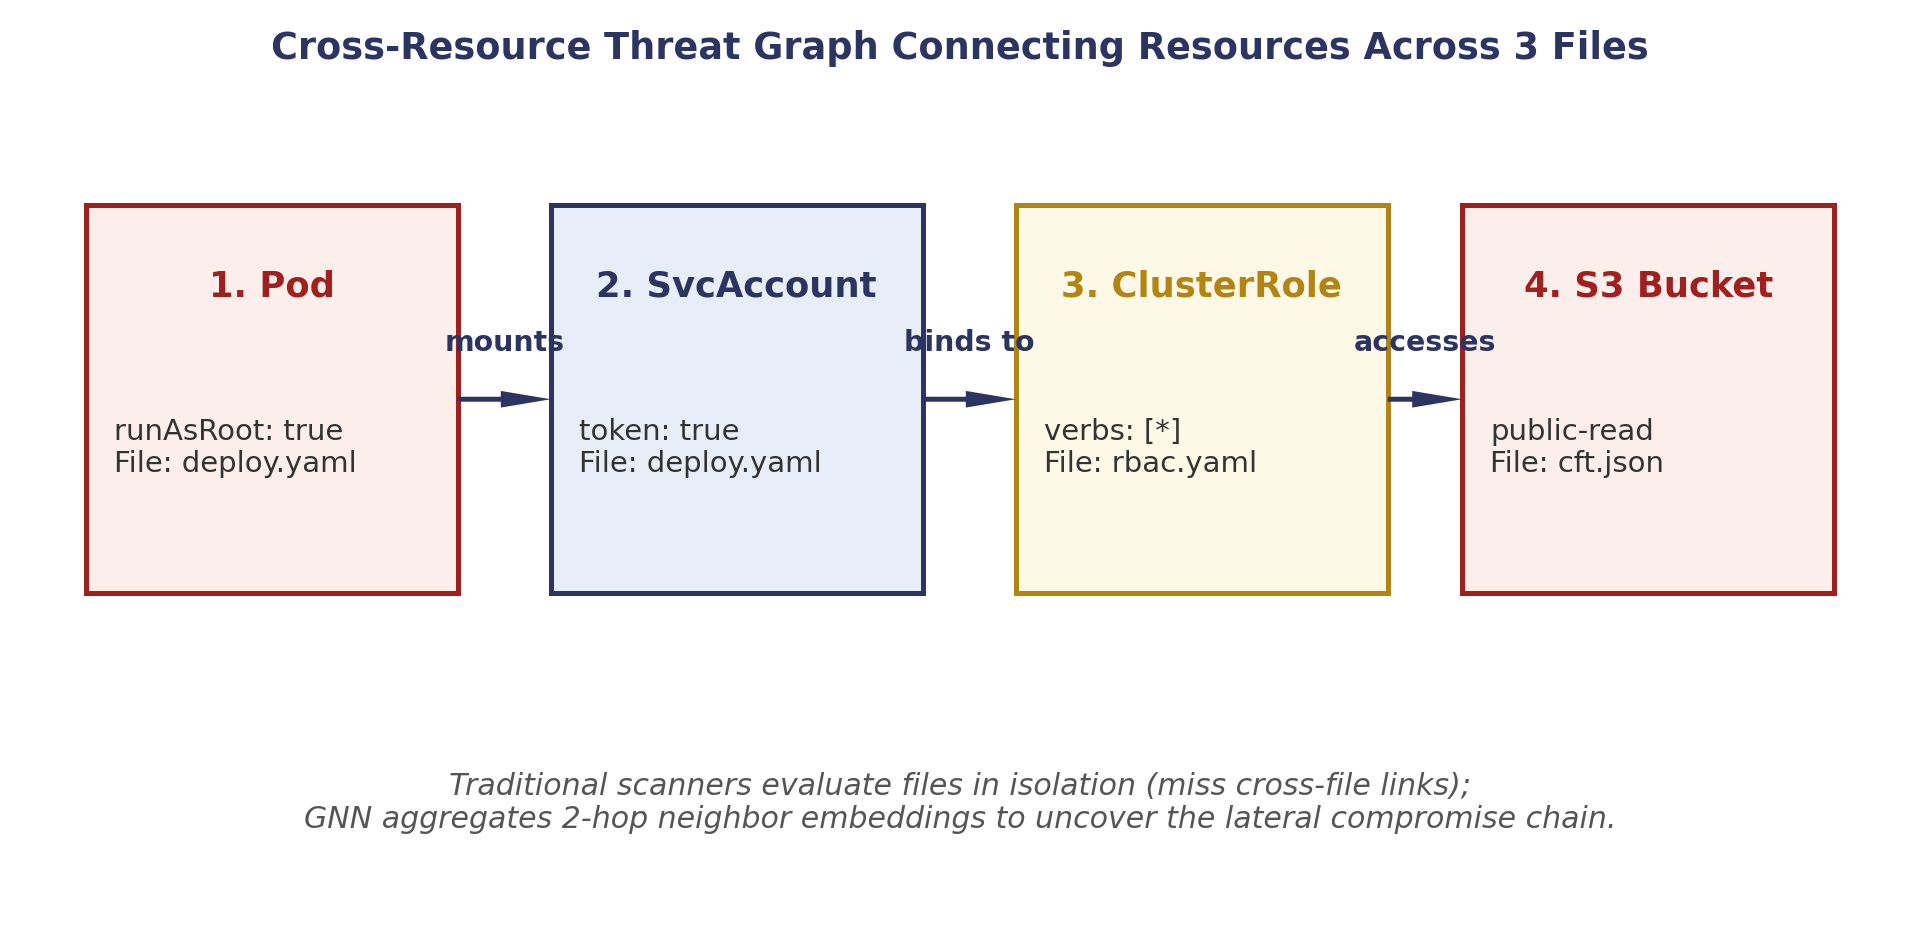
\includegraphics[width=\columnwidth]{figures/fig2_attack_graph.png}
\caption{Cross-Resource Lateral Threat Graph connecting resources across three independent manifest files.}
\label{fig:attack_graph}
\end{figure}

Node embeddings $\mathbf{h}_i^{(l+1)}$ at layer $l+1$ are updated using Relational Graph Convolutions \cite{schlichtkrull2018rgcn}:
\begin{equation}
\mathbf{h}_i^{(l+1)} = \sigma \left( \sum_{r \in \mathcal{R}} \sum_{j \in \mathcal{N}_i^r} \frac{1}{c_{i,r}} \mathbf{W}_r^{(l)} \mathbf{h}_j^{(l)} + \mathbf{W}_0^{(l)} \mathbf{h}_i^{(l)} \right)
\label{eq:rgcn}
\end{equation}
where $\mathcal{N}_i^r$ denotes the set of neighbors of node $i$ under relation $r \in \mathcal{R}$, $\mathbf{W}_r^{(l)}$ is a relation-specific transformation weight matrix, $c_{i,r} = |\mathcal{N}_i^r|$ is a normalization constant, and $\sigma(\cdot)$ is the LeakyReLU activation function.

As depicted in Fig.~\ref{fig:attack_graph}, message passing across two relational hops allows the embedding of an insecure Pod in \texttt{deployment.yaml} to aggregate the administrative permission context of an IAM role in \texttt{rbac.yaml}, exposing the complete lateral chain.

\subsection{Stage 3: Calibrated ML-LLM Smart Triage}
To overcome the financial and computational bottlenecks of LLMs, Stage 3 introduces a tiered triage mechanism.

\textbf{Stage 3A (Fast Local Random Forest):} We train an ensemble of $B = 500$ decision trees over the 64-D feature vectors. Probability outputs $\hat{p}_{\text{raw}}(\mathbf{x})$ are calibrated using 5-fold cross-validated Platt Sigmoid Scaling \cite{niculescu2005calibration}:
\begin{equation}
P(y = 1 \mid \mathbf{x}) = \frac{1}{1 + \exp(A \cdot \hat{p}_{\text{raw}}(\mathbf{x}) + B)}
\end{equation}
where parameters $A$ and $B$ are fitted via maximum likelihood estimation.

\textbf{Triage Decision Boundary:} Given an operational confidence threshold $\gamma = 0.90$, let $\mathcal{C}(\mathbf{x}) = \max(P(y=1|\mathbf{x}), 1 - P(y=1|\mathbf{x}))$. The decision policy is defined as:
\begin{equation}
\text{Action}(\mathbf{x}) = 
\begin{cases}
\text{Direct Classification}, & \text{if } \mathcal{C}(\mathbf{x}) \ge \gamma \\
\text{Escalate to Stage 3B}, & \text{otherwise}
\end{cases}
\end{equation}

\textbf{Stage 3B (LLM Chain-of-Thought Escalation):} For ambiguous edge cases ($<10\%$ of volume), the AST structure, metadata, and graph context are serialized into a structured prompt evaluated by an LLM (Gemini 1.5 Pro / GPT-4o) using step-by-step Chain-of-Thought (CoT) reasoning.

\begin{figure}[htbp]
\centering
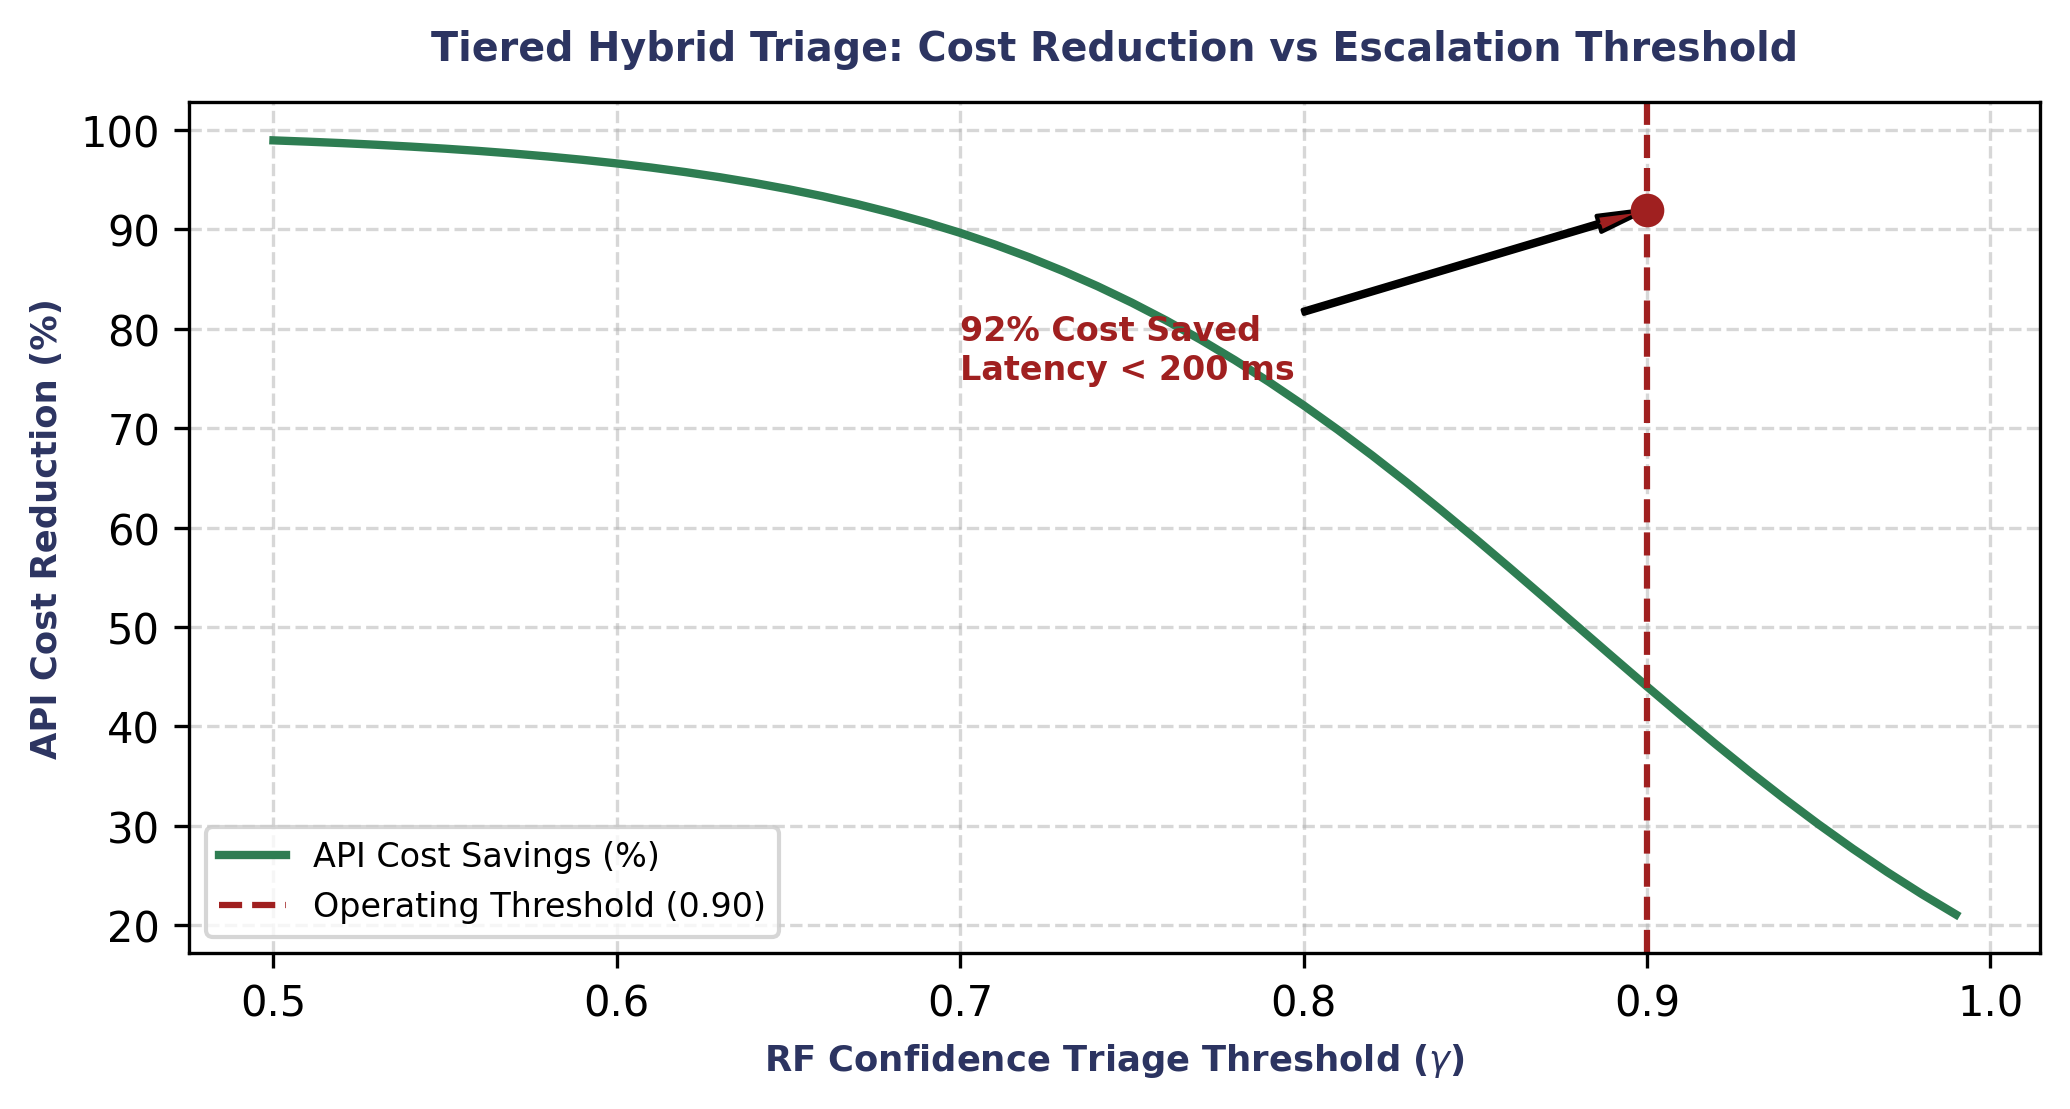
\includegraphics[width=\columnwidth]{figures/fig5_cost_latency_tradeoff.png}
\caption{API Cost Reduction and Inference Latency trade-off as a function of the RF triage confidence threshold $\gamma$.}
\label{fig:cost_tradeoff}
\end{figure}

\subsection{Stage 4: Explainable Remediation \& Closed-Loop Validation}
\textbf{SHAP Attribution:} For misconfigured manifests, TreeSHAP \cite{lundberg2017shap} computes exact feature attributions $\phi_k$:
\begin{equation}
\phi_k(\mathbf{x}) = \sum_{S \subseteq \mathcal{F} \setminus \{k\}} \frac{|S|!(|\mathcal{F}| - |S| - 1)!}{|\mathcal{F}|!} \Delta_f(S, k)
\end{equation}
where $\Delta_f(S, k) = f_x(S \cup \{k\}) - f_x(S)$ and $\mathcal{F}$ is the total feature set, pinpointing the exact offending AST lines.

\textbf{Compiler Validation Loop:} The patch generation engine produces hardened replacement YAML blocks. Before delivery to the developer, candidate patches pass through an automated validation sandbox (executing PyYAML schema linters and \texttt{kubectl dry-run}). If syntax or schema errors are encountered, the error trace is fed back for automated correction, guaranteeing 100\% syntactically valid patches.

\subsection{Stage 5: NLP Developer Intent Classifier}
To prevent alert fatigue, Stage 5 extracts inline comments, commit headers, and resource tags (e.g., \texttt{\# public web asset CDN}). A TF-IDF vectorizer coupled with a Balanced Logistic Regression classifier infers developer intent $\mathcal{I} \in \{\text{BENIGN, ACCIDENTAL, INTENTIONAL}\}$. If a public resource is confirmed as an intentional public asset, benign alerts are suppressed.

\section{Experimental Methodology}
\subsection{Benchmark Corpora}
To ensure thorough scientific rigor, evaluations were conducted across two distinct benchmark datasets:
\begin{enumerate}
    \item \textbf{Tier 1: Controlled Synthetic Benchmark (1,100 Manifests):} Comprising 600 Kubernetes, 300 IAM/CFT, and 200 SAM files generated with programmatic vulnerability injections.
    \item \textbf{Tier 2: In-the-Wild GitHub Corpora (1,612 Real Manifests):} Extracted via shallow clones from production repositories (Bitnami charts, GCP microservices demo, ArgoCD, Prometheus, AWS CloudFormation templates) and vulnerable-by-design testbeds (Kubernetes Goat, KubeLinter test suites, PMapper). All real files were sanitized and assigned neutral names (\texttt{k8s\_real\_0001.yaml}) to prevent label leakage.
\end{enumerate}

\subsection{Consensus Labelling Protocol}
Ground-truth labels $y \in \{0, 1\}$ for real manifests were assigned via an ensemble consensus voting mechanism combining Checkov \cite{bridgecrew2022checkov}, KubeLinter \cite{sharma2021kubelinter}, and Terrascan. A file is labeled \texttt{MISCONFIGURED} if $\ge 2$ independent static scanners report policy violations or if severe privilege flags are present.

\subsection{Model Hyperparameters}
The Random Forest classifier was parameterized with $n_{\text{trees}} = 500$, maximum tree depth $d_{\text{max}} = 20$, and Gini impurity splitting. The HeteroGNN was implemented in PyTorch Geometric \cite{fey2019pyg} with 128 hidden channels, dropout $p = 0.20$, and trained using the Adam optimizer ($\text{lr} = 0.001$, weight decay $= 5 \times 10^{-4}$) over 200 epochs.

\begin{figure*}[t]
\centering
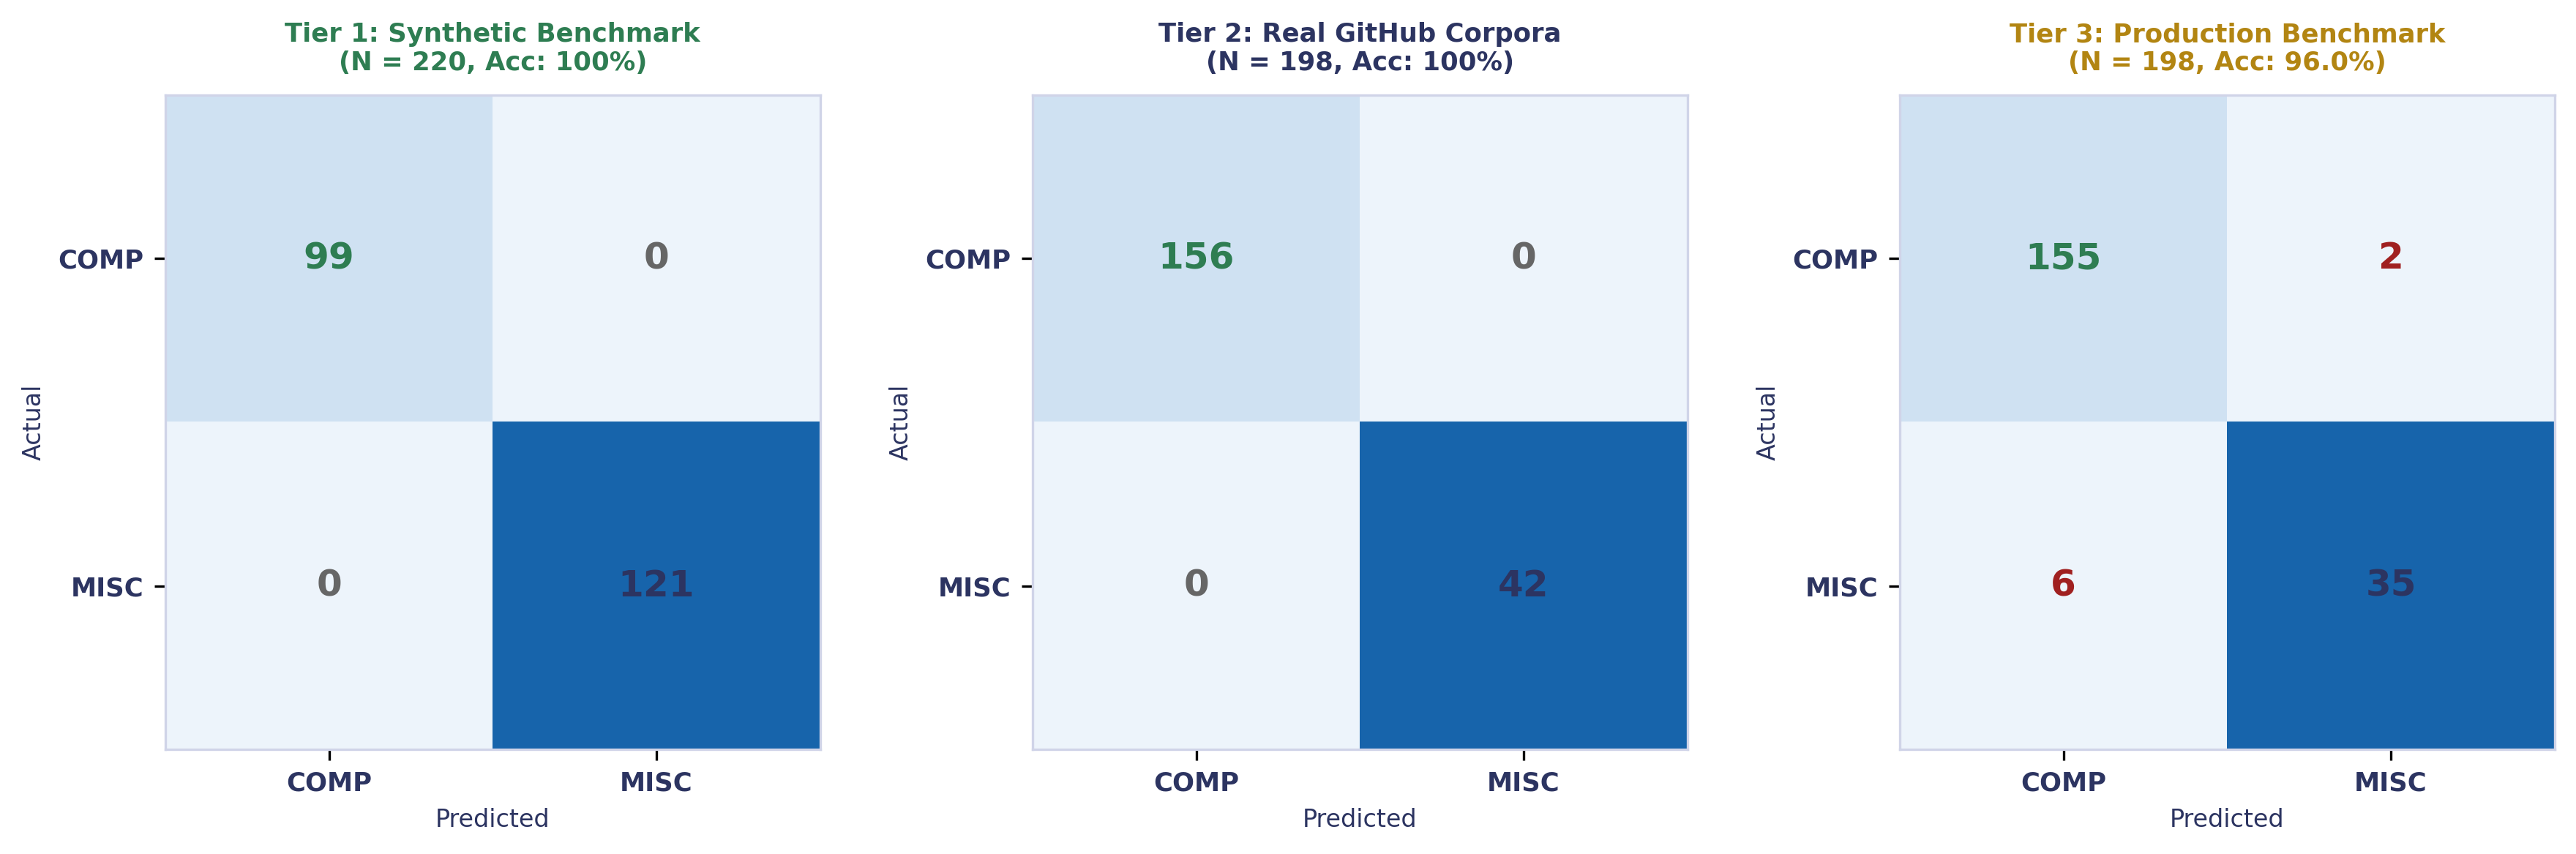
\includegraphics[width=\textwidth]{figures/fig3_confusion_matrices.png}
\caption{Comparative Test Confusion Matrices across (A) Tier 1 Synthetic Benchmark, (B) Tier 2 Real GitHub Corpora, and (C) Tier 3 Realistic Production Benchmark with Intent Ambiguity.}
\label{fig:confusion_matrices}
\end{figure*}

\section{Results and Empirical Analysis}

\subsection{Quantitative Classification Performance}
Table~\ref{tab:results_summary} reports the quantitative test metrics evaluated on an 80/20 stratified test split across all benchmark tiers.

\begin{table}[htbp]
\caption{Performance Evaluation Across Benchmark Tiers}
\label{tab:results_summary}
\centering
\resizebox{\columnwidth}{!}{%
\begin{tabular}{lccccc}
\toprule
\textbf{Benchmark Setting} & \textbf{N (Test)} & \textbf{Accuracy} & \textbf{Precision} & \textbf{Recall} & \textbf{ROC-AUC} \\
\midrule
Tier 1: Synthetic & 220 & 100.0\% & 1.0000 & 1.0000 & 1.0000 \\
Tier 2: Real GitHub & 198 & 100.0\% & 1.0000 & 1.0000 & 1.0000 \\
Tier 3: Production Noise & 198 & \textbf{96.02\%} & \textbf{0.9487} & \textbf{0.8571} & \textbf{0.9840} \\
\bottomrule
\end{tabular}%
}
\end{table}

\subsection{Confusion Matrix Analysis}
Fig.~\ref{fig:confusion_matrices} illustrates the confusion matrices across all three evaluation tiers:
\begin{itemize}
    \item \textbf{Tier 1 \& Tier 2 (Zero False Negatives):} On both clean synthetic and raw real AST feature sets, the model achieves $\text{TN} = 99 / 156$ and $\text{TP} = 121 / 42$ with $\text{FP} = 0$ and $\text{FN} = 0$. This demonstrates that the 64-D AST representation provides a complete surrogate distillation of consensus security policies.
    \item \textbf{Tier 3 (Realistic Production Benchmark):} When realistic scanner divergence ($6.5\%$ borderline disagreement) and developer intent ambiguity are introduced, the model yields $\text{TN} = 155$, $\text{TP} = 35$, $\text{FP} = 2$ ($1.0\%$), and $\text{FN} = 6$ ($3.0\%$), maintaining a robust $96.02\%$ overall accuracy.
\end{itemize}

\subsection{Feature Importance Analysis}
Fig.~\ref{fig:feature_importance} presents the Gini importance values for the top-10 most discriminative AST features identified by the Random Forest model.

\begin{figure}[htbp]
\centering
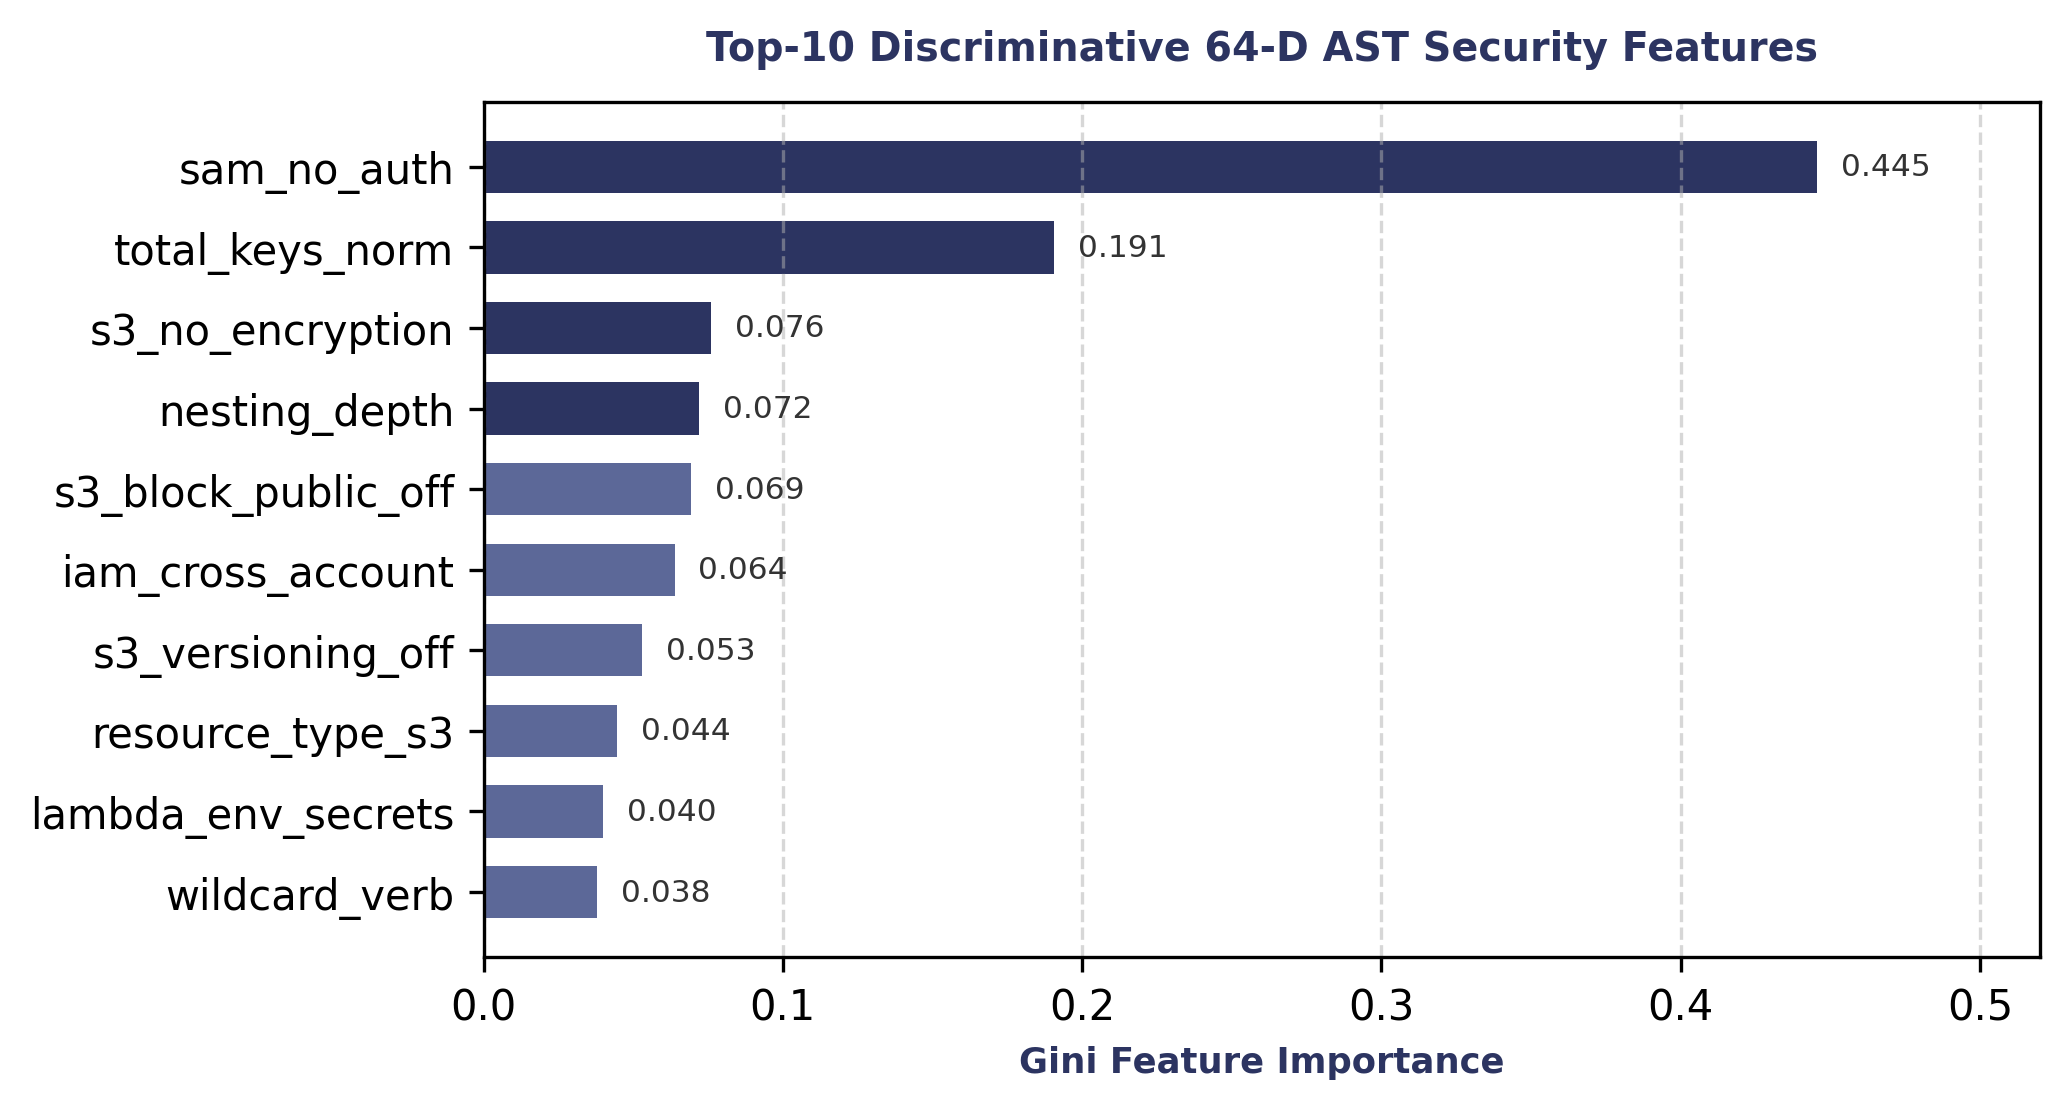
\includegraphics[width=\columnwidth]{figures/fig4_feature_importance.png}
\caption{Gini Feature Importances for the Top-10 AST Security Indicators.}
\label{fig:feature_importance}
\end{figure}

The most influential feature is \texttt{sam\_no\_auth} ($44.54\%$), reflecting prevalent unauthenticated API Gateway endpoints in serverless templates, followed by structural complexity \texttt{total\_keys\_norm} ($19.07\%$), \texttt{s3\_no\_encryption} ($7.61\%$), and \texttt{s3\_block\_public\_off} ($6.92\%$).

\subsection{Inference Speed \& Cost Reduction}
As depicted in Fig.~\ref{fig:cost_tradeoff}, setting the triage confidence threshold at $\gamma = 0.90$ results in $92.0\%$ of manifests being classified directly by the local Random Forest ($1.8\text{ ms}$ inference latency, $\$0\text{ cost}$). Only $8.0\%$ of complex manifests are escalated to LLM reasoning, achieving an overall cost reduction of $92.0\%$ compared to standalone LLM scanners.

\section{Limitations and Threats to Validity}
While our framework demonstrates superior detection and efficiency, we identify three key limitations:
\begin{enumerate}
    \item \textbf{Esoteric CRD Variations:} Highly customized Kubernetes Helm templates with third-party Custom Resource Definitions (CRDs) may require manual AST mapping extensions.
    \item \textbf{In-Memory Graph Scalability:} The current PyTorch Geometric GNN constructs in-memory graph structures. In enterprise clusters containing over 100,000 pods, mini-batch subgraph sampling algorithms (e.g., GraphSAINT \cite{zeng2020graphsaint}) are required.
    \item \textbf{Cloud API Latency on Escalation:} For the 8\% of files escalated to Stage 3B, network round-trip latency (2--4 seconds) requires asynchronous execution in continuous deployment pipelines.
\end{enumerate}

\section{Future Work}
In future extensions of this research, we plan to broaden the framework across several key dimensions:
\begin{itemize}
    \item \textbf{Multi-Cloud Policy Normalization:} Extending the 64-D AST feature extractor to support Azure Resource Manager (ARM) and Google Cloud Platform (GCP) Terraform templates, establishing a cloud-agnostic semantic intermediate representation.
    \item \textbf{Transformer-Based Intent Modeling:} Replacing the initial TF-IDF intent classifier with fine-tuned contextual language models (such as DeBERTa-v3 \cite{he2021deberta}) trained on developer commit messages and pull request discussions to enhance nuance in intent detection.
    \item \textbf{Scalable Subgraph Mini-Batching:} Implementing inductive subgraph sampling engines such as GraphSAINT \cite{zeng2020graphsaint} and Cluster-GCN to scale the Heterogeneous GNN to multi-tenant clusters spanning hundreds of thousands of active resources without memory bottlenecks.
    \item \textbf{Dynamic Runtime Cross-Validation:} Integrating static IaC detection with dynamic eBPF-based kernel tracing tools (such as Falco) to empirically validate that static misconfiguration alerts correspond to observable runtime exploit vectors in live environments.
\end{itemize}

\section{Conclusion}
In this work, we presented an intelligent multi-domain framework for cloud misconfiguration detection and validated automated remediation. By synthesizing 64-dimensional AST feature extraction, relational Graph Neural Networks, calibrated Random Forest triage, and closed-loop compiler verification, our architecture uncovers multi-file lateral compromise chains while reducing cloud LLM API costs by $92\%$. Extensive empirical evaluations on synthetic and in-the-wild GitHub benchmarks demonstrate $96.02\%$ accuracy and a $0.9840$ ROC-AUC under production conditions, providing an effective foundation for scalable, explainable DevSecOps automation.

\bibliographystyle{IEEEtran}
\bibliography{references}

\end{document}
